\clearpage
\section{Example Legal Graph}
\label{appendix:legal-graph}

Figure~\ref{fig:appendix-retirement-age-graph} shows the retirement-age topic
as a concrete graph example. A complete answer may require moving from the Labor
Code provision to the implementing decree and then to the appendix table that
contains year-specific retirement ages.

\begin{figure}[H]
  \centering
  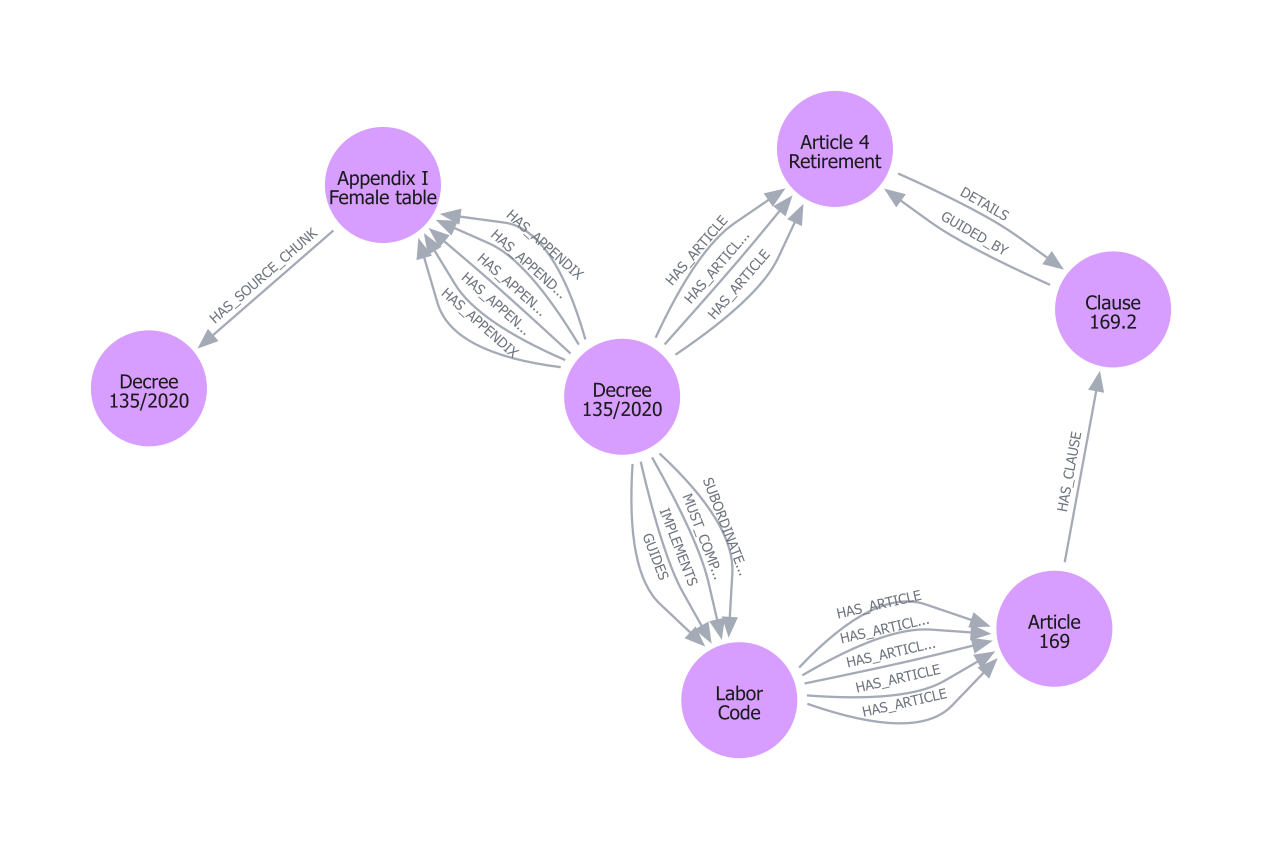
\includegraphics[width=0.92\textwidth]{figures/retirement-age-graph-cropped.png}
  \caption{Example legal graph expansion for retirement-age evidence.}
  \label{fig:appendix-retirement-age-graph}
\end{figure}

The graph uses the actual implementation labels and relationship types shown
below.

\begin{ThesisCode}
Labels:
Legal_Document, Legal_Article, Legal_Clause,
Legal_Appendix, Evidence_Chunk

Relationships:
HAS_ARTICLE, HAS_CLAUSE, HAS_APPENDIX, HAS_SOURCE_CHUNK,
DETAILS, GUIDED_BY, IMPLEMENTS, GUIDES, MUST_COMPLY_WITH,
SUBORDINATE_TO
\end{ThesisCode}
